% Annual Cognitive Science Conference

\documentclass[10pt,letterpaper]{article}

\usepackage{cogsci}
\usepackage{pslatex}
\usepackage{apacite}
\usepackage{graphicx}
\usepackage{amsmath,amssymb}
\usepackage[longnamesfirst]{natbib}
\usepackage{url}

\title{Representing and Learning a Large System of Number Concepts \\ with Latent Predicate Networks}
 
\author{
  {\large \bf Joshua Rule (rule@mit.edu)}\\
  {\large \bf Eyal Dechter (edechter@mit.edu)}\\
  {\large \bf Joshua B. Tenenbaum (jbt@mit.edu)}\\
  MIT, 46-4053, 77 Massachussetts Avenue, Cambridge, MA 02139 USA}

\begin{document}

\maketitle

\begin{abstract}
  Conventional models of concept learning represent the challenge of
  learning as one of choosing and labeling individual concepts from a
  possibly infinite set of options ({\bf CITATIONS NEEDED}). They tend
  to underemphasize the fact that we learn many concepts as part of
  large, potentially infinite, systems rather than as isolated
  individuals. In such cases, the challenge of learning is not so much
  in providing a single, stand-alone definition for a concept, but in
  describing the richly structured relationships between concepts. The
  natural numbers are one of the first such abstract conceptual
  systems children acquire, and psychologists have accordingly spent
  decades investigating number knowledge in children and adults as a
  case study in concept representation and acquisition
  \citep{fuson1988children,galGel2005,Car2009}. Even so, models of
  natural number learning have largely ignored two challenges related
  to the language-like productivity and compositionality of exact
  number concepts: 1) there is an unbounded set of exact number
  concepts, each with distinct semantic content; and 2) people can
  reason flexibly about any of these concepts (even fictitious ones
  like \emph{eighteen-gazillion and thirty-one}). Conventional models
  of concept learning focused on representing individual concepts as
  collections of prototypes or rules do not naturally explain these
  capacities. Models must instead learn the structure of the entire
  infinite set of exact number concepts, focusing on how relationships
  between numbers support reference and generalization. Here, we
  suggest that the latent predicate network (LPN) -- a probabilistic
  context-sensitive grammar formalism -- facilitates tractable
  learning and reasoning for exact number concepts
  \citep{DecRulTenming}. We show how the number words and their
  relations to one another can be expressed in this formalism and
  discuss a Bayesian learning algorithm for LPNs, suggesting a
  computational mechanism by which children might learn abstract
  numerical knowledge from linguistic utterances about numbers.

  \textbf{Keywords:}
  child development; concept learning; number; generalization;
  computational model; grammar induction;
\end{abstract}

\section{Introduction}

Humans seldom learn isolated concepts; they more frequently appear as
part of a system. We learn about noses by constrasting them with eyes
and mouths, and about red by constrasting it with green and blue. The
natural numbers (1, 2, 3, $\ldots$) are no exception: to understand a
number such as \emph{one}, we must not only learn to ground it by
relating it to concepts and percepts we already know, but we must also
relate it to other number concepts we are still in the process of
acquiring. The natural numbers are in fact particularly interesting in
this respect because they are infinite -- there is no way to learn all
the individual concepts without learning the structure of the entire
system.

A great deal of empirical work has focused on the first part of this
problem, on how the first few number concepts are grounded in counting
routines and the core systems of approximate magnitude and parallel
object individuation ({\bf CITATIONS}). Recent studies have also
proposed computational mechanisms to explain several key behavioral
changes during early number learning ({\bf CITATION}).

Significantly less work has been done, however, on the second half of
the problem, on how concepts are learned as systems and partially
defined with respect to each other. While the problems of how children
link physical sets with the counting routine and develop their first
number concepts are crucial, we direct our attention elsewhere in this
paper. We focus on how children might acquire knowledge of an infinite
number system, particularly for numbers which they are unlikely to
ever see counted out explicitly.

We share a common interest with the recent family of Rational Rules
models
\citep{goodman2008rational,T.D.Ullman:2012:1b1b6,PianGoodTen2012} in
exploring concept learning through Bayesian induction of compositional
representations using sparse evidence. We agree that these points are
fundamental to understanding concept learning. The major difference is
in how our models represent concepts; both use a grammar, but for
different purposes. Rational Rules models see concepts as specific
sentences generated according to a grammar. The (potentially infinite)
hypothesis space over specific concepts is a collection of all
sentences generated by that grammar, and the goal is to find sentences
which apply to collections of objects in the world. In the model we
present here, the hypothesis space is not over sentences in a grammar
but over possible grammars. Moreover, neither these grammars nor
sentences in this grammar represent individual concepts. It is instead
the entire language of the grammar, the network of all possible
sentences or relations which, taken as a whole, describes certain
concepts. Where Rational Rules models see concepts as specific
sentences in a grammatical language, our approach views concepts as
networks of grammatically-generated relations.

We begin by discussing how to represent the sort of conceptual
knowledge needed to describe an infinite number system, and ashow how a
particular formalism, the Probabilistic Range Concatenation Grammar
(PRCG) can represent number this way \citep{boullier2005range}. We
then show how this grammar can be learned using Bayesian inference in
an LPN, a learning framework for PRCGs \citep{DecRulTenming}.

\section{Representing Number Knowledge}

To show how a system of concepts like number might be learned, we must
first understand what that system of concepts is and how it might be
represented. This task is non-trivial for number learning, and several
models have been proposed. For example,
\citeauthor{hurford1975linguistic} (\citeyear{hurford1975linguistic})
describes a single system differentiating primitive and compound
number concepts, while \citeauthor{siegler1982development}
(\citeyear{siegler1982development}) propose a system with several
stages of development, each of which contains little internal
structure.

To motivate our stance on the issue, we begin by describing several
challenges a representation of number must overcome. We then formally
introduce PRCGs as an answer to these challenges. Finally, we show how
this formalism, initially developed to explain syntactic structures in
natural language, can explain the conceptual structure of number
words.

\subsection{The Challenges of Number}

Relative to many other semantic fields children encounter ({\it e.g.}
the parts of the body, types of furniture in a house), the natural
numbers are highly distinctive.

First, where many semantic fields refer to relatively concrete classes
of objects or object parts, the natural numbers refer primarily to an
abstract property (cardinality) of an abstract entity (sets). Semantic
fields like the parts of the body also tend to be relatively limited
in scope, applying primarily, in this case, to physical parts of
animals. By contrast, natural number is incredibly broad, applying not
only to concrete objects, but also to things like other sets ({\it
  e.g.} three pairs of socks), sounds, events, time periods, people
and other agents, and numbers themselves ({\it e.g.} three threes
makes nine).

Second, there are infinitely many number concepts. Even given a
practically infinite number of instantiated body parts ({\it e.g.}
Timmy's nose), the collection of names for body parts is small ({\it
  e.g.} tail, eye, nose, tummy, ...). By contrast, not only are there
a practically infinite number of natural number instances ({\it e.g.}
three noses), but a truly infinite number of natural number concepts
({\it e.g.} three). Moreover, being infinite, the amount of explicitly
counted, perceptually-grounded evidence children receive relative to
the size of the semantic field is incredibly sparse (When did you last
see exactly 253 objects?) In order to accommodate such an expressive
conceptual system in a finite mind, the concepts themselves must be
constructed as needed in a systematic and compositional manner.
Being infinite and broadly applicable also suggests that numbers can
be learned, represented, and understood without direct perceptual
grounding.

Third, numbers do not uniquely describe cardinalities for children but
initially have distinct meanings related to sequencing, counting,
measuring, ordinality, and several non-numerical meanings ({\it e.g.}
telephone numbers) (Fuson, Richards, Briar, 1982). Even when numbers
do describe cardinalities, interest may not be so much in the
cardinality itself as in some more complex property, such as whether
it is more or less than another cardinality or how it operates
arithmetically via addition, subtraction, multiplication, or division.
Indeed, children may eventually learn about negative and rational
numbers, algebra, geometry, and myriad other mathematical disciplines.
This hugely diverse range of meanings makes it impossible to fully
describe the meaning of \emph{three} without referencing \emph{two},
\emph{four}, and eventually all other numbers. The concept of
\emph{two} (or any other number) is not rightly understood as a single
object, but must also include the web of relationships in which
\emph{two} participates.

How can we hope to represent a systems of concepts which are: 1)
learnable without direct perceptual grounding; 2) compositionally
constructed; and 3) relationally defined? Happily, these properties
are similar to those many computatonal linguists have faced in
studying natural language syntax. Motivated by this similarity, we
will use a grammar to represet the system of natural number concepts.
Grammars can be induced directly from a stream of utterances, are
highly compositional, and define their constituents based on their
relationships to each other rather than as discrete objects. While
most work in natural language syntax is context-free, our focus on
capturing structural relationships in concepts demands that we use a
context-sensitive grammar. Specifically, we choose to use Range
Concatenation Grammars (RCGs), an expressive, context-sensitive
formalism in which reasoning remains relatively tractable ({\bf
  CITATION}).

\subsection{A Grammar for Number Concepts}

\begin{figure*}[t]
  \begin{centering}
    \includegraphics[width=0.9\linewidth]{grammarOfNumber/gon.pdf}
    \caption{A Range Concatenation Grammar whose strings are valid number words.}
    \label{fig:gon}
  \end{centering}
\end{figure*}

\begin{figure*}[t]
  \begin{centering}
    \includegraphics[width=\linewidth]{parseTrees/parse.pdf}
    \caption{RCG parses for \emph{Number} (Blue), \emph{Successor} (Red), and \emph{More} (Green).}
    \label{fig:parse}
  \end{centering}
\end{figure*}

Having motivated our decision to model concepts as sets of relations
expressed by a grammar, and having described RCGs as our formalism of
choice, we now present the grammar of number knowledge we have
constructed. In this initial exploration, we have captured five key
number relations: \emph{Number}, capturing the distinction between
valid and invalid number words; \emph{Succ} and \emph{Pred}, the
successor and predecessor relations, respectively; and \emph{More} and
\emph{Less} the more-than and less-than relations, respectively. While
seemingly basic tasks, they take years to master
\citep{FusRicBriar1982}.

Capturing these relations with an RCG is not only possible, but it can
be done quite compactly. Our grammar for the concepts of
\emph{Number}, \emph{Successor}, \emph{Predecessor}, \emph{Less}, and
\emph{More} covers all numbers between 0 and 1 billion, exclusive, and
requires only 216 rules. Even considering just \emph{Number},
\emph{Successor}, and \emph{Predecessor}, these 216 rules cover more
than 500 quadrillion relations. Figure \ref{fig:gon} shows a schematic
of the rules concerned with determining valid and invalid numbers,
while the rest, due to space constraints, can be found
online.\footnote{http://github.com/joshrule/GrammarInduction}

Two notes of clarification: First, our grammar never produces nor
parses full English sentences. This is a grammar for the structure of
concepts, not the structure of language. When attempting to parse
something like \emph{Succ(ninety nine, one hundred)}, we assume some
other system more directly involved in language preprocesses
utterances into a partially predicated state, which is then checked
against the knowledge encoded in our conceptual grammar. Second, this
grammar has not been optimized for compactness or efficiency. A number
of predicates could be compressed or even eliminated, for example, by
implementing \emph{More} with a binary search tree or as the
transitive closure of \emph{Successor}. Instead, we focused on
providing a grammar that would be correct, easy to understand for the
human reader, and fit a prefix-base-suffix understanding of number, as
discussed below.

Intuitively, a number word like \emph{six-hundred thirty-seven} is
valid because we have six units of one hundred each and thirty-seven
remaining units of one each. That is, we have some base unit (hundred)
and we track both how many of them we have (six), and how many of the
next smallest base unit (one) we have (thirty-seven). We denote the
sum of these (six-hundred + thirty-seven) simply by concatenating the
two terms from largest to smallest base (six-hundred thirty-seven).
This structure is recursive. \emph{Nine-thousand seven-hundred
  sixteen} is created by taking nine thousands units and tacking on a
remainder, which is seven hundreds plus its remainder of sixteen ones:
\emph{nine} $\times$ \emph{thousand} $+$ (\emph{seven} $\times$
\emph{hundred} + (\emph{sixteen} $\times$ \emph{one})). Note that
there is no explicit mention of the base \emph{one} in a valid number
word - it is implied and marked by appending $\varnothing$, the empty
string, instead of \emph{one}.

Our grammar similarly uses a prefix-base-suffix system, and figure
\ref{fig:parse} shows how our grammar concludes that \emph{six-hundred
  thirty-seven} is a valid number word. As with our intuitive example
above, we must show that \emph{six} is a valid prefix for
\emph{hundred} and \emph{thirty-seven} is a valid suffix (Number(six
hundred thirty seven) $\leftarrow$ Prefix(six,hundred),
Suffix(thirty,seven)). We must show that our use of the largest base
is legal, as well as show recursively that the rest of the number is
legal. \emph{Six} is a valid prefix for \emph{hundred} because it is a
number word representing a \emph{ones} number, a number between one
and nine (Prefix(six,hundred) $\leftarrow$ Ones(six)). It would be
incorrect for \emph{hundred} to have no prefix, and it would also be
incorrect to use a prefix larger than \emph{nine}. \emph{Thirty-seven}
is a valid suffix because it is a valid number for a previous base, in
this case $\varnothing$, the ones base (Suffix(hundred,thirty seven)
$\leftarrow$ LargerBase(hundred,$\varnothing$), Number(thirty seven)).
\emph{thirty-seven} is one of these numbers because it is merely the
concatenation of a \emph{decade} word and a \emph{ones} word
(Number(thirty seven) $\leftarrow$ Prefix(thirty seven,$\varnothing$),
Suffix($\varnothing$,$\varnothing$), and Prefix(X Y,$\varnothing$)
$\leftarrow$ Decades(X), Ones(Y)). Thus, the compositional use of
simple predicates helps us analyze the structure of a complex phrase
like \emph{six hundred thirty seven} and show that while it is a valid
number word, \emph{hundred six seven thirty} is not. \emph{Successor}
and \emph{More} can similarly be encoded (Figure \ref{fig:parse}),
while \emph{Predecessor} and \emph{Less} can be encoded quite simply
as $\text{Less}(X,Y) \leftarrow \text{More}(Y,X)$ and
$\text{Pred}(X,Y) \leftarrow \text{Succ}(Y,X)$.

\section{Learning Number Knowledge}

How might children learn the knowledge about number that is captured
in the representation presented above? In this section, we present a
computational model of learning over RCGs and take a first step
towards evaluating this model against the learning trajectories and
patterns of error reported in the literature on counting. 

Because the learning problem is computationally challenging and
because much of the focus in the literature on exact number knowledge
has been on counting, we restrict our experiments here to the
successor relation, and, in particular, to learning how to count from
one to a hundred.

Learning to count up to a hundred does not come easily. Studies of
counting in children between three and six years of age, suggests that
although some children are able to count up to a hundred shortly
before entering kindergarten, many have trouble with the task at least
as late as first
grade~\cite{FusRicBriar1982,miller1987counting}. These studies suggest
that children do not learn to count to a hundred by memorizing the
sequence of numbers between on and a hundred. As might be expected of
a system that will eventually be able to count to arbitrarily large
numbers, learning to count to a hundred involves discovering the
pattern that successive number words follow. 

We will model this process of pattern discovery as probabilistic
inference over RCGs and show that the generalization phenomena
described in these studies is captured by this model. 

\subsection{Latent Predicate Networks}

\begin{figure}[t]
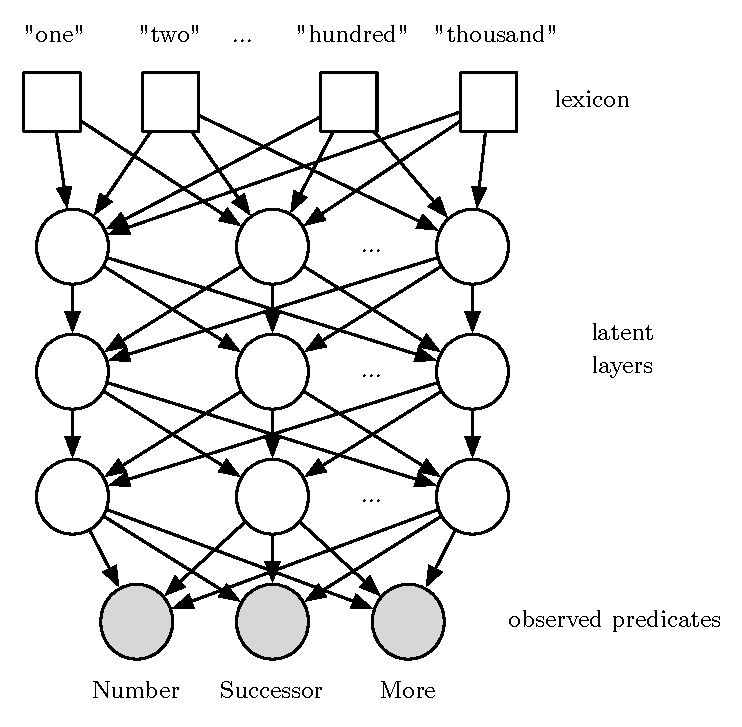
\includegraphics[width=0.9\linewidth]{figures/lpn}
\caption{A schematic LPN for number knowledge learning.}
\end{figure}

Latent Predicate Networks (LPNs) are PRCGs with a large number of
rules connected in a layered fashion. An schematic of the LPN used in
the following learning experiments and simulations is show in
Figure~\ref{fig:lpn}. There are three types of predicates in LPNs. The
\emph{observed} predicates are relations that are directly present in
the data (e.g. the successor predicate Succ is observed if the data is
a collection of successor pairs). The observed predicates are defined
in terms of layers of \emph{latent} predicates. These are relations
that are not directly observable in the data and whose meanings are
determined through learning. For example, the Decade predicate, which
is true for ``ten'', ``twenty'', etc., might correspond to one of the
latent predicates after learning on successor pair data. The lowest
layer of latent predicates is defined in terms of a collection of
\emph{lexicon} predicates, each of which is a unary predicate that is
true of the atomic units (the words) of the system.

Given a collection of observations, our model assumes that there is a
setting of the parameters of the LPN that gave rise to those
observations. The model's goal is to infer what those parameters
are. This inference is conducting via hierarchical Bayesian
inference~(CITATION): the model assumes that there is a prior
distribution over the parameters of the LPN and that given those
parameters the LPN induces a distribution over observations. Using
Bayes' rule, the model infers a distribution over parameter values
that balances the fit of the observations against the prior. We use a
sparsity inducing prior distribution which formalizes the intuition
that latent predicates and rules should be shared in order to learn
grammars that can generalize beyond the observed data.

Exact inference in probabilistic grammars is computationally
intractable. We use the common ``variational'' approximation
implemented using Variational Bayes EM algorithm~(CITATION), which has
been widely used in approximate inference of probabilsitic context
free grammars~(CITATION). All the computations in this paper were done
using the PRISM probabilistic logic programming language~(CITATION).

All the simulations below were run on an LPN with three layers of five
predicates each. The learning algorithm was run for a single
iteration, a concentration parameter $alpha=0.1$, and a convergence
criterion of $\epsilon=1e-4$.

\subsection{Modeling the acquisition and elaboration of the count sequence}

\citet{FusRicBriar1982} describe qualitative phenomena of
count sequence acquisition and elaboration based on several surveys in
which they asked American children between three and five years of age
to count (either while counting a collection of objects or just
reciting the count world sequence). The learning trajectories and
error patterns they describe have inspired computation modeling
efforts using connectionist networks; for example,
\citet{ma1989modeling} use an associative network to model the errors
that young children typically make when learning the count sequence up
to twenty or thirty. But, to our knowledge, such models have not been
used to study how children acquire the count sequence beyond twenty.


\begin{figure*}[t]
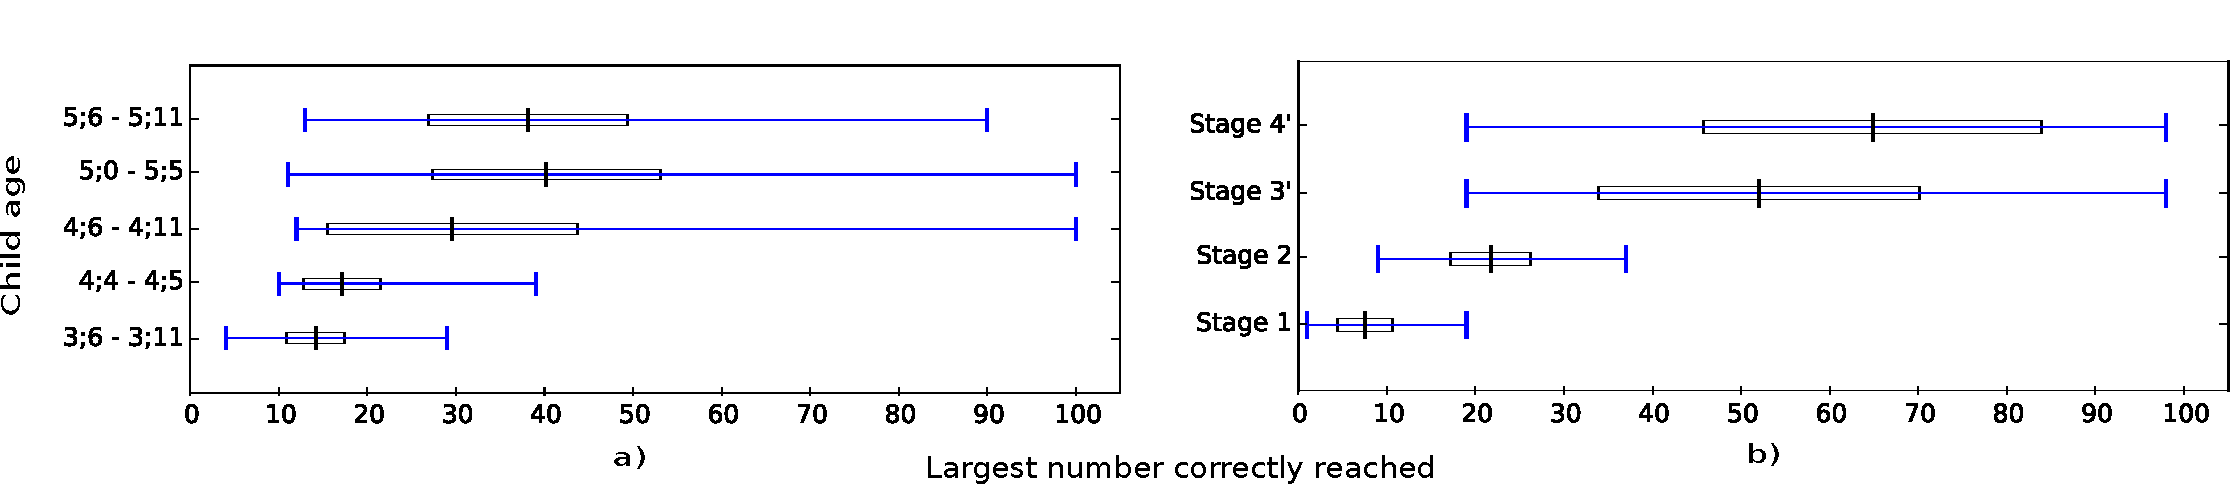
\includegraphics[width=0.9\linewidth]{figures/modelboxplot}
\caption{Data from~\citet{FusRicBriar1982} on children's ability to
  recite the count list. The x-axis shows the highest number correctly
  reached when children were asked to count starting at ``one.'' Boxes
  correspond to the standard deviation, central bands to the means,
  and the whiskers to the range.
\label{fig:fuson_count_data}}. 
\end{figure*}

Figure~\ref{fig:fusonTable} shows the highest number correctly reached
by children in various age ranges~\cite{FusRicBriar1982}. The authors
hypothesize that the large jump in range between the young three year
olds and the older four year olds and year olds is due to the older
children partially solving what they term ``the decade problem.'' --
i.e. recognizing both that there is a repetitive pattern of that
repeats across decades beyond twenty and learning that there is a
particular sequence to the decade words.

We asked whether our model goes through a similar transition. To
simulate learning, we generated data sets consisting of successor
pairs between one and a hundred, with the number of examples of each
pair $Succ(i+1, i)$ following the power law $N=\frac{K}{i}$, where $K$
determines the overall size of the data set. To simulate the different
overall quantities of data that children are exposed to by different
ages, we generated data sets for $K=10, 100, 1000, 10000$. The
resulting histograms of data are shown in
Figure~\ref{fig:counting_grid}a-d (the y-axes are logarithmically
scaled). 

For each of these data sets we ran our learning algorithm ten times,
generating ten simulated children at each stage (the simualations
differ due to different random parameter intiailizations). In
Figure~\ref{fig:counting_grid}a-d, each line corresponds to one of the
simulated children and shows the probability that the child will
correctly count to the corresponding number on the x-axis. To generate
this counting simulations, we asked the model for the distribution of
successors for a given number and used a simple soft max decision procedure
to determine the probability of the simulated child reporting each
word. Specifically, the p(

\begin{figure*}[t]
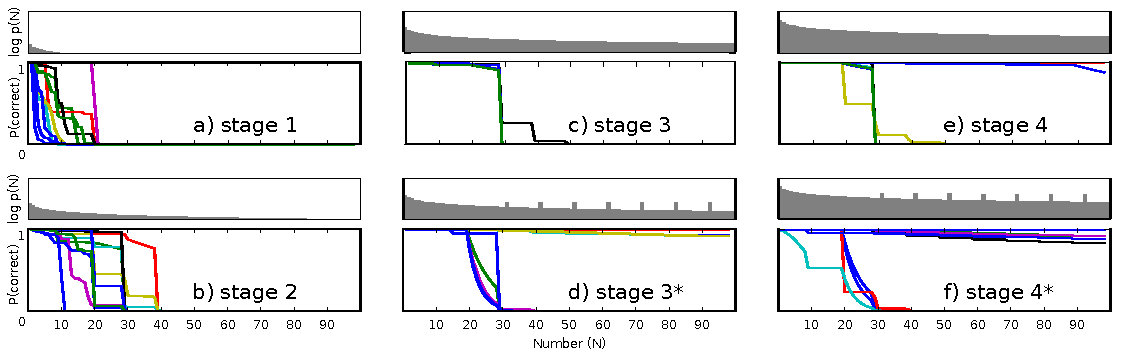
\includegraphics[width=\linewidth]{figures/counting_grid2}
\caption{Our model's performance correctly reciting the count sequence
  having learned with various quantities and types of evidence. Each
  line corresponds to a single run of the learning algorithm given the
  distribution of data shown in the histogram directly above it. For
  each number along the x-axis the y-axis corresponds to the
  probability that model correctly counts from one up to that
  number. The y-axes on the data histograms are shown on a logarthmic
  scale. The simulations in a) were trained on the least data and
  those in b-d) on increasing quantities of data. Those in e) and f)
  were trained on the same data as those in c) and d), respectively,
  with the modification that extra emphasis was placed on the decade
  transitions. \label{fig:counting_grid}}
\end{figure*}


\begin{figure}
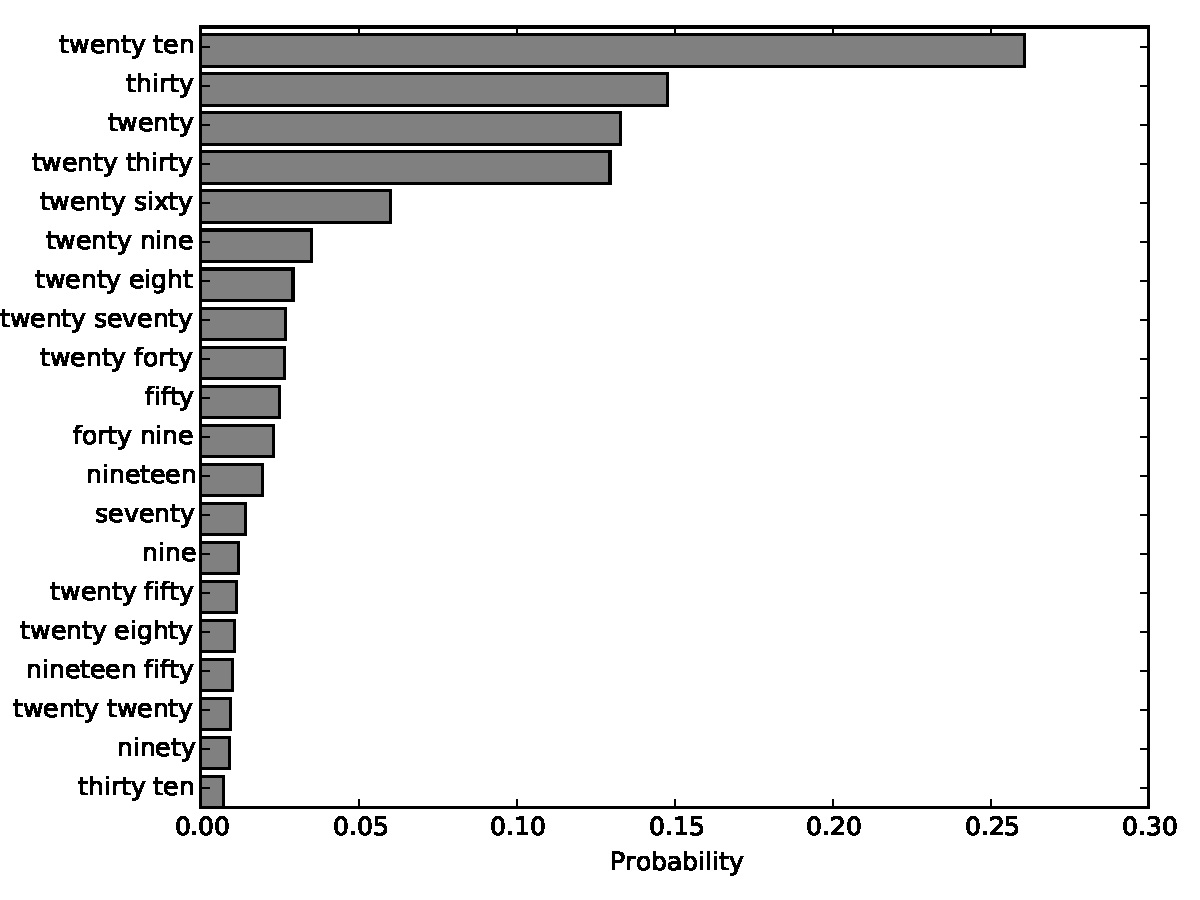
\includegraphics[width=0.9\linewidth]{figures/after29}
\caption{The distribution over successors of ``twenty nine'' given learning on the evidence corresponding to Figure~\ref{fig:counting_grid}b. \label{fig:after29}}
\end{figure}


\begin{figure}
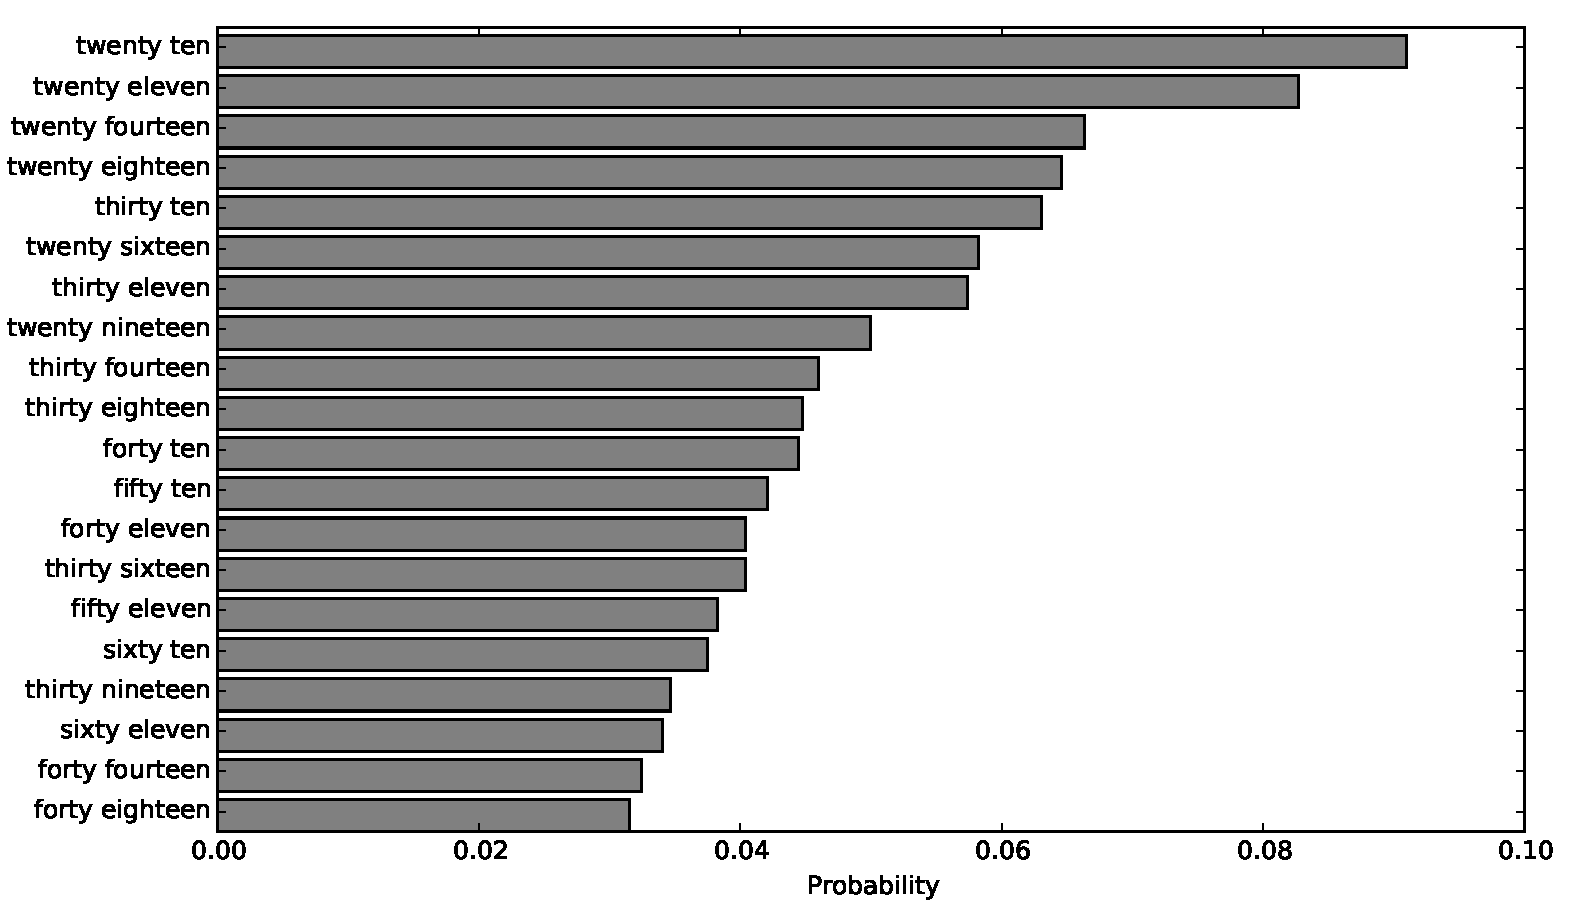
\includegraphics[width=0.9\linewidth]{figures/inventedWords}
\caption{The distribution over invented words for simulated child
  learner at stage
  3 (see Figure~\ref{fig:counting_grid}c). \label{fig:inventedWords}}
\end{figure}


\section{Discussion}

%% first half: Eyal

Either way, as these models claim to cover more well-trodden
territory, they should also become correspondingly more quantitative
in their predictions. The ability to generalize as well as the
qualitative similarities we show here between LPNs and children's
overgeneralizations are intriguing, but 

%% second half of discussion

While the conceptual grammar contains a great deal of knowledge about
\emph{fifty-two}, there is no object that in any sense contains the
entire meaning of \emph{fifty-two}. That meaning is defined by the
collection of relationships which hold for the token \emph{fifty-two}.
In a similar vein, the names given to specific predicates in our
grammar are arbitrary. \emph{Number} could just as easily be called
\emph{Yulmpa} or \emph{Snarg}. What is important is not a predicate's
name, but the relations it enters into with other predicates and thus
the argument strings for which it holds. The same is true for
individual words like \emph{hundred} or \emph{nine}: while any name
could be used, what cannot be changed is the way each predicate
combines or contrasts a given token with other tokens in the grammar.
{\bf THEORY-THEORY and how all concepts are defined as relations
  between entities?}

As mentioned in the introduction, the LPN model of concept learning
shares many similarities with the Rational Rules family of models
\citep{goodman2008rational,T.D.Ullman:2012:1b1b6,PianGoodTen2012},
particularly our focus on learning concepts from sparse evidence using
Bayesian induction over compositional representations. We differ in
how we use grammars. Rational Rules models use a grammar to generate
sentences, each of which represents a single concept to be learned.
LPNs, by contrast, learn a grammar which generates relations, each of
which describes a particular interaction between a set of concepts.

For example, the Rational Rules-based model of Cardinal Principle (CP)
learning given in \citep{PianGoodTen2012} is focused on finding a
specific sentence which captures the CP, in this case a program in the
simply-typed lambda calculus. An LPN-based approach would be to learn
a complete grammar over many number concepts, the relationships
between some of which happen to correctly encode the CP.

Note, however, that this paper focuses on a different psychological
problem than Piantadosi and colleagues (\citeyear{PianGoodTen2012}) in
that we are not proposing a model of how children acquire or ground
their initial number concepts or the CP. Neither our hand-crafted nor
our learned \emph{Number} predicates contain any link between set
cardinalities and number words, nor does \emph{More} connect in any
way to approximate magnitude. We intend to explore these connections
in future work but focus here on the fact that to know what the number
words mean is to know how they interact with each other as well as
concepts you already have, including (potentially innate) pre-existing
conceptions of \emph{More} or \emph{Less} used to differentiate sets,
or the version of \emph{Successor} used to memorize songs and
routines.

That said, we see no fundamental incompatibility between the model
presented here and extensions to include approximate magnitude, object
tracking, set manipulation, more complex morphology ({\it e.g.} the
meaning of \emph{-illion} or \emph{-teen}), or different counting
strategies ({\it e.g.} as used in Turkish, French, or Mandarin) as
would be needed for a more comprehensive model of number learning. Far
from it, we see our work here as a first demonstration of LPN's
suitability for capturing a broad range of number concepts, though
whether more general models are best approached by working strictly
within the LPN formalism or by using it as one module within a more
complex framework is an open question. Certainly, the human mind is
more powerful than an RCG and is at least Turing-complete. RCGs
provide a tractable way, however, to explore a restricted subclass of
problems. The strategies and solutions we discover here are also
available in Turing-complete systems, and in fact implemented in one
(PRISM Prolog) so our findings easily generalize to more expressive
grammars.

More broadly, we see this paper as growing out of the hypothesis that
much of human learning, including the explosion of knowledge that
occurs during development, can be explained as induction in a formal
language. This vision of the \emph{child-as-hacker} draws on and
extends the notion of the \emph{child-as-scientist}; not only are
children forming theories about the world, but they are simultaneously
developing the very conceptual language they use to formulate those
theories.

% Boullier 2003 shows that RCGs can compute things as sophisticated
% as prime number detection, though by very different means than we
% use here. Even so, understanding how to bring these abilities into a
% symbolic or mixed symbolic/iconic system is an open question.
% similar to Boullier, 2003 in that the interest is in using RCGs to
% capture mathematical concepts. The approach taken here is very
% different though. We're using a fully symbolic, rather than an
% iconic, representation of number. Boullier's work may be
% informative, though for understanding approximate magnitudes and
% other iconic forms of representation.

\section{Acknowledgments}

The authors benefited significantly from conversations with Timothy
O'Donnell and Leon Bergen. This material is based upon work supported
by the Center for Minds, Brains and Machines (CBMM), funded by NSF STC
award CCF-1231216, an NSF Graduate Research Fellowship, and the Eugene
Stark Graduate Fellowship.


\bibliographystyle{apacite}

\setlength{\bibleftmargin}{.125in}
\setlength{\bibindent}{-\bibleftmargin}
\bibliography{cogsci}

\end{document}



%% Despite this pivotal role, current evidence suggests humans are
%% born without an innate understanding of the natural numbers
%% \citep{Car2009}. Number is instead laboriously acquired over the
%% course of early childhood, a process stretching well into grade school
%% \citep{Nat2010}. Even so, the natural numbers are among the first
%% abstract, symbolic conceptual systems we acquire. Understanding how
%% number is acquired -- on what basis representation and by what
%% computational process -- is far more than a simple case study and
%% promises to significantly increase our understanding of abstraction
%% and conceptual development.
%% 
%% Natural number acquisition has accordingly been studied intensely and
%% to great effect. Infant and animal studies suggest several innate
%% systems, while not containing explicit natural number concepts, are
%% important for scaffolding our initial representations of number. These
%% include systems for object individuation and approximate magnitude
%% \citep{feigenson2004core,dehaene2011number}. One of the most
%% well-established phenomena of number learning is that the ability to
%% reliably count sets of objects develops stereotypically, even among
%% cultures where number is traditionally unimportant
%% \citep{Wyn1992,JarPianSpelEtAl2014}. Initially, people are
%% completely unable to associate sets of a given size with the correct
%% number word. Then, they can do so for sets no larger than one,
%% followed much later by sets no larger than two, followed again by
%% sets no larger than three. Typically, children then appear to
%% generalize the procedure to the other number words they know and can
%% reliably count out sets of any size, provided they know a sufficiently
%% large count list. At this point, they are said to have acquired the
%% \emph{Cardinal Principle} and are variously called \emph{CP-knowers}
%% or \emph{full counters}.
%% 
%% Attempts to collate decades of number research into a coherent model
%% have largely focused on the cognitive change that helps children
%% become \emph{full counters} \citep{Car2009,PianGoodTen2012}. Recent
%% work suggests, however, that the ability to reliably count sets of
%% objects, while closely related, is undeniably distinct from our
%% conceptual knowledge of numbers as representing cardinalities of exact
%% sets \citep{DavEngBar2012,izard2014toward,JarPianSpelEtAl2014}. More
%% generally, counting a set of objects requires only a very partial
%% understanding of number. Models of counting and number learning have
%% also focused almost exclusively on numbers between one and ten,
%% presumably because it is during this interval that children become
%% \emph{full counters}. Most studies, then, examine the development of a
%% specific skill requiring limited knowledge of a small subset of
%% numbers.
%% 
%% While the problems of how children link physical sets with the
%% counting routine and develop a concept of sets as exact collections
%% are crucial, we direct our attention elsewhere in this paper. We focus
%% on how children might acquire knowledge of an infinite number system,
%% particularly for numbers which they are unlikely to ever see counted
%% out explicitly. We begin by discussing how to represent the sort of
%% conceptual knowledge needed to describe an infinite number system, and
%% show how a particular formalism, the Probabilistic Range Concatenation
%% Grammar (PRCG) can represent number this way
%% \citep{boullier2005range}. We then show how this grammar can be
%% learned using Bayesian inference in an LPN, a learning framework for
%% PRCGs \citep{DecRulTenming}.
